\documentclass{scrartcl}
\usepackage[utf8]{inputenc}
\usepackage[frenchb]{babel}
\usepackage{amssymb}
\usepackage{lmodern}
\usepackage[T1]{fontenc}
\usepackage{hyperref}
\usepackage{verbatim}
\usepackage{listings}
\usepackage{graphicx}

\usepackage{color}
\definecolor{deepblue}{rgb}{0,0,0.5}
\definecolor{deepred}{rgb}{0.6,0,0}
\definecolor{deepgreen}{rgb}{0,0.5,0}

\newcommand{\brokencell}[2][c]{\begin{tabular}[#1]{@{}c@{}}#2\end{tabular}}

\lstset{frame=single, breaklines=true,
          breakatwhitespace=true, basicstyle=\scriptsize,
          showstringspaces=false, escapeinside={(*}{*)},
          keywordstyle=\color{deepblue},
          stringstyle=\color{deepred},
          commentstyle=\color{deepgreen},
          literate=
                   {é}{{\'e}}1{É}{{\'E}}1
                   {è}{{\`e}}1{È}{{\`E}}1
                   {ê}{{\^e}}1{Ê}{{\^E}}1
                   {à}{{\`a}}1{À}{{\`A}}1
                   {ù}{{\`u}}1{Ù}{{\`U}}1
                   {û}{{\^u}}1{Û}{{\^U}}1
                   {ô}{{\^o}}1{Ô}{{\^O}}1
                   {ó}{{\'o}}1{Ó}{{\'O}}1
                   {ç}{{\c c}}1{Ç}{{\c C}}1
                   {œ}{{\oe}}1{Œ}{{\OE}}1
        }

\begin{document}
\title{Rapport du projet de théorie des jeux}
\author{Maxence Ahlouche \and Maxime Arthaud \and Korantin Auguste
          \and Martin Carton \and Thomas Forgione \and Thomas Wagner}
\date{11 novembre 2013}
\maketitle
\tableofcontents
\newpage

\section{Présentation de l'équipe}
  Cette équipe a été menée par Thomas Forgione, assisté de son Responsable
  Qualité Maxence Ahlouche. Les autres membres de l'équipe sont Martin Carton,
  Thomas Wagner, Maxime Arthaud, et Korantin Auguste.

  Tous les membres de l'équipe ont été présents à chacune des séances lors de
  cette UA.

\section{Shifumi}
    Une stratégie simple et efficace à laquelle on pourrait penser pour gagner
    au Shifumi serait de jouer de manière aléatoire.

    Et en effet, il s'avère que si les deux joueurs jouent de manière équiprobable,
    on a affaire à un équilibre de Nash: aucun changement de stratégie de la part
    d'un joueur ne pourra lui permettre d'augmenter ses chances de gagner.

    De plus, si un adversaire ne joue pas de manière aléatoire (ou augmente les
    probabilités de jouer un certain élément), alors on pourra prévoir ce qu'il
    va jouer et donc trouver une stratégie qui pourra le battre. Les humains
    étant très mauvais pour jouer de manière aléatoire, il est assez facile
    d'écrire une stratégie permettant de les battre.

  \subsection{Stratégie développée}
    Afin de démontrer qu'un adversaire ne jouant pas aléatoirement est facile
    à battre, nous avons développé une stratégie qui se base sur des chaînes
    de Markov: en se basant sur les derniers éléments joués, elle regarde
    dans l'historique pour voir l'élément qui était joué le plus souvent par
    l'adversaire après les derniers coups joués.

    Cette stratégie s'avère vraiment efficace contre un joueur humain.
    Toutefois, elle est prévisible: si on sait qu'on a affaire à une telle
    stratégie, on peut jouer de manière à la battre.

    C'est pour cela qu'une stratégie aléatoire est la seule pouvant maximiser
    nos gains dans le pire des cas.

  \subsection{Variantes}
    Toutes les variantes du Shifumi qui consistent à rajouter des éléments
    pour obtenir un nombre d'éléments pair (par exemple
    pierre/papier/ciseaux/puits) vont créer un déséquilibre, car un élément
    sera moins efficace contre les autres. L'équilibre de Nash du jeu va
    alors consister à ne jamais jouer cet élément.

    Si le nombre d'éléments est impair, alors le jeu pourra être équilibré,
    comme un Shifumi classique.

  \subsection{Tests}
    TODO

\section{Jeu de la somme magique}

\subsection{Représentation sous forme de morpion}
Ce jeu, comme expliqué dans les transparents présentés en cours,
consiste à choisir, à tour de rôle, $n$ nombres parmi $n^2$ afin que
leur somme soit égale à $\frac{n(n^2+1)}{2}$.

Une représentation possible de ce jeu est le carré magique: les
joueurs doivent choisir, l'un après l'autre une case dans un carré
magique, leur but étant de contrôler une ligne, une colonne ou une
diagonale entière du carré magique; alors, les nombres qu'ils auront
choisis totaliseront le score voulu. De même, ce problème correspond exactement
au jeu du morpion, étendu à des grilles $n \times n$.

Ainsi, une des stratégies possibles pour un joueur du jeu de la somme
magique est de construire un carré magique, et de représenter les
nombres choisis par l'adversaire par un rond dans la case
correspondante. Afin de choisir un nombre, il suffit d'appliquer la
stratégie de morpion de son choix sur le carré magique, et de
jouer le nombre correspondant.

Le choix du carré magique n'importe pas. En effet, dans un carré
magique sont présentes toutes les possibilités de combinaison de
nombres pour obtenir la somme voulue. Par conséquent, peu importe le
carré magique d'ordre $n$ que l'on choisit, les représentations sous forme de
morpion seront toutes équivalentes.

Le morpion étant un jeu où l'on essaie de minimiser la perte maximum,
on peut s'intéresser à l'algorithme du minmax, pour déterminer une
stratégie non-perdante.

\subsection{Algorithme du minmax appliqué au jeu du morpion}
L'algorithme du minmax consiste à évaluer toutes les positions de jeu
atteignables depuis la position courante, sur une certaine profondeur
(autrement dit, un certain nombre de tours de jeu), et à jouer de
manière à atteindre la position la plus avantageuse, en supposant que
l'adversaire joue toujours le meilleur coup pour lui-même (ce coup
étant évalué avec notre propre fonction d'évaluation, qui n'est pas
forcément la même que celle de l'adversaire).

Par conséquent, afin d'implémenter l'algorithme du minmax, il faut
commencer par déterminer une fonction d'évaluation.

\subsubsection{Fonction d'évaluation}
La fonction d'évaluation que nous avons choisie est très simple: une
ligne, colonne ou diagonale (que nous appelleront désormais simplement
``ligne'') complétée avec notre symbole (ce qui signifie qu'on a
gagné) vaut $+\infty$; si, au contraire, l'adversaire a complété une
ligne, alors cette ligne vaut $-\infty$. Une ligne contenant
uniquement notre symbole rapporte le nombre d'occurrences de notre
symbole dans cette ligne ; à l'inverse, une ligne contenant uniquement
le symbole de l'adversaire rapportera négativement le nombre
d'occurrences de ce symbole dans cette ligne.
Toutes les autres lignes ne rapportent aucun point.
Ainsi, l'évaluation d'une position de jeu est la somme des points
rapportés par chacune de ses lignes, colonnes et diagonales.

\subsubsection{Minmax}
L'algorithme du minmax va construire (implicitement) l'arbre des coups
possibles à partir de la position courante.
L'évaluation d'un nœud de cet arbre sera:
\begin{itemize}
  \item si c'est à notre tour de jouer, le maximum de l'évaluation de nos fils;
  \item si c'est à l'adversaire de jouer, le minimum de l'évaluation
    de ses fils (i.e.\ on suppose que l'adversaire joue le meilleur
    coup à sa disposition, selon la fonction d'évaluation du joueur courant).
\end{itemize}

L'évaluation d'une feuille de l'arbre se fera par la fonction
d'évaluation définie précédemment.

Ainsi, l'algorithme se dirigera naturellement vers la position la plus
avantageuse pour lui.

\subsection{Élagage alpha-bêta}
L'élagage alpha-bêta permet de réduire le nombre de nœuds à parcourir durant
l'algorithme du minmax.

Cette algorithme arrête le parcours des fils d'un nœud quand il se rend
compte qu'il ne pourra pas faire mieux.

Dans l'exemple suivant, où les nœuds en bleus sont ceux où l'on doit prendre
le minimum, et ceux en gris le maximum :
\begin{center}
  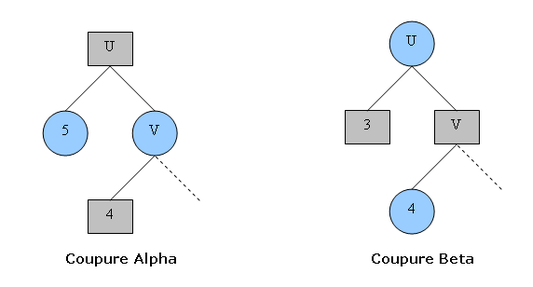
\includegraphics[width=300px]{coupures_alpha-beta.png}
\end{center}

On se rend bien compte qu'on n'a pas besoin de parcourir les nœuds suivant,
car on prend le maximum des minimums, ou l'inverse.

Par exemple, pour la coupure alpha : si on trouve des fils de $V$ plus petit
que $4$, on va prendre le maximum, donc c'est $4$ qui sera utilisé, et si on
trouve plus grand ou égal à $5$, on devra prendre le minimum au niveau de $V$,
donc on prendra $5$ dans tous les cas.

Au final, cette amélioration permet de gagner un temps considérable.

\subsection{Résultats}
\subsubsection{Meilleure stratégie}
Nous avons fait s'affronter différentes stratégies les unes contre les
autres, afin de voir laquelle était la meilleure, sur différentes
tailles de plateaux. Les stratégies que nous avons fait s'affronter
étaient:
\begin{itemize}
  \item la stratégie aléatoire,
  \item la stratégie qui prend toujours la première case disponible,
  \item les stratégies utilisant le minmax à différentes profondeurs,
    entre 2 et 10,
  \item les stratégies utilisant le minmax et l'élagage alpha-bêta à
    différentes profondeurs, entre 2 et 10.
\end{itemize}
Les résultats ne sont guère surprenants: toutes les stratégies
parviennent au match nul, à l'exception des stratégies aléatoires et
premier\_dispo, qui perdent systématiquement contre un minmax de
profondeur supérieure à 2.

\subsubsection{Performances}
Du point de vue du temps d'exécution, toutefois, l'algorithme avec
élagage est beaucoup plus rapide qu'un minmax simple, alors qu'il
retourne le même résultat.
Malheureusement, nous n'avons pas pu tester nos algorithmes sur des
plateaux de grande taille: en effet, à partir de la taille 4, un
minmax avec élagage de profondeur 10 met en moyenne 5 secondes pour
décider de son coup, et peut aller jusqu'à 40s!

Il est également intéressant de noter, bien que ceci n'ait rien à voir
à notre projet, que le passage du langage Python au langage C a permis
de diviser le temps d'exécution des tests par 60 pour des stratégies
sans élagage.

\section{Compétition/Duopole}
  Le but de ce jeu est de maximiser le gain d'une entreprise en concurrence
  avec une autre entreprise en fonction de leur production.

  \subsection{Analyse}
    Notre gain étant égal à $g_x(x) = -x(x+y-3)$ avec $x$ et $y$ les
    productions respectives des deux entreprises, pour le maximiser il
    suffirait de jouer $x=\frac{3-y}{2}$ (c'est que fait la stratégie fournie
    \verb+noncooperatif+).
    
    Cependant au moment de décider quelle quantité produire nous ne connaissons
    pas la production $y$ de l'entreprise concurrente. De plus si les deux
    entreprises s'ignorent totalement en essayant de maximiser leur seul gain,
    elles gagneront au final moins que deux entreprises qui coopèrent
    totalement c'est à dire qui chercheraient à maximiser leur gain total
    $g_x(x)+g_y(y)$ avec $g_x(x) = g_y(y)$ c'est à dire en jouant $x=y=0.75$.
    En effet, elles gagneront alors chacune $\frac 9 8$ à chaque tour au lieu
    de $1$ si elles sont toutes les deux non-coopératives.

    Nous avons donc essayé plusieurs stratégies différentes, qui essayent de
    maximiser le gain de l'entreprise en tenant en compte l'autre entreprise,
    les productions et les gains des tours précédents.

  \subsection{Stratégies}
    \subsubsection{Stackelberg}
      Une variante de la stratégie Stackelberg consiste à utiliser la
      production moyenne de l'autre joueur plutôt que seulement la dernière
      valeur. Elle permet d'obtenir des résultats légèrement meilleurs.

      De plus en coopérant avec l'autre joueur (voir listing~\ref{lst:mmmttk})
      si celui-ci coopère, on obtient de meilleurs résultats.

      Enfin, une autre variante de cette stratégie (voir
      listing~\ref{lst:mmmttkv2}) maximise le gain si l'autre joueur a joué une
      constante sur les derniers tours. Cette variante donne des résultats
      un peu moins bons en moyenne mais est meilleure dans le meilleur des cas.

    \subsubsection{Stratégie pénalisante}
      Le principe de cette stratégie (voir listing~\ref{lst:penalise}) est
      d'être coopératif tant que l'adversaire l'est, et de devenir plus
      agressif quand il ne l'est plus: à chaque fois que l'autre joueur n'est
      pas coopératif, on joue comme le ferait la stratégie Stackelberg.

      Une variante de cette stratégie (voir listing~\ref{lst:penaliseviolent})
      consiste à le pénaliser de plus en plus: la première fois on le pénalise
      une fois, puis deux, puis trois, etc.

      Ces deux stratégies sont efficaces à la fois quand l'autre joueur est
      coopératif (on est alors coopératif) et contre un joueur non-coopératif
      (on devient alors agressif).

    \subsubsection{Stratégie évolutive}
      Une autre stratégie (voir listing~\ref{lst:pokemon}) que nous avons
      développée consiste à augmenter la production si la dernière augmentation
      a augmenté notre gain ou si la dernière diminution l'a diminué et
      vice-versa.

      Celle-ci est plutôt efficace, mais n'est pas la meilleure que nous ayons
      développée: elle se met souvent à osciller inutilement.

    \subsubsection{Stratégie polynomiale} \label{sec:poly}
      Enfin, une autre stratégie (voir listing~\ref{lst:poly}) joue en fonction
      de la production moyenne de l'autre joueur telle que:
      \begin{itemize}
        \item $f(0) = 1.125$: on joue beaucoup si l'autre joue peu, sans jouer
          trop pour ne pas le fâcher;
        \item $f(0.75) = 0.75$: elle coopère avec quelqu'un qui coopère;
        \item $f(1.5) = 0.75$: elle coopère avec quelqu'un qui ne coopère pas,
          pour essayer de faire coopérer celui-ci (c'est dans notre intérêt et
          ça ne changerait pas son gain, il est donc possible qu'elle le
          fasse).
      \end{itemize}

      On choisit alors la fonction $f$ pour être un polynôme qui interpole ces
      valeurs.

      Cette méthode s'avère très efficace en moyenne.

  \subsection{Comparaison}
    Les tables~\ref{table:coop_results} et~\ref{table:coop_results2} montrent
    les résultats obtenus par les quelques stratégies que nous avions à notre
    disposition\footnote{Les stratégies fournies par les professeurs
    (marquées~*), les notre et des stratégies «~prêtées~» par d'autres
    groupes pour les tests (marquées~**) que nous remercions.} pour une durée
    de $99$ tours et $1000$ tours respectivement. Nous faisons s'opposer toutes
    les stratégies entre elles puis notons pour chacune d'elles son gain
    minimal, moyen et maximal\footnote{Cette table peut être générée par le
    script matlab \textit{comp\_tests.m} fourni dans l'archive.}.

    %Todo: mettre à jour avec les dernières valeurs quand on aura fini et mettre
    %les résultats pour un autre nombre de tours: il suffit d'appeler
    %\verb+comp_tests(100, true)+ d'ajouter les * et les $\backslash$\_ et
    %supprimer cette phrase quand on aura fini.
    \begin{table}[f]
      \centering
      \begin{tabular}{|c||c|c|c|}
        \hline
        Stratégie      & Gain minimal & Gain moyen & Gain maximum \\\hline\hline
           cooperatif* & $ 55.31$ & $ 97.84$ & $111.38$ \\\hline
        noncooperatif* & $ 42.96$ & $ 87.74$ & $130.26$ \\\hline
          stackelberg* & $ 48.00$ & $ 79.75$ & $114.69$ \\\hline
                palkeo & $ 15.75$ & $ 92.49$ & $111.38$ \\\hline
              Pénalise & $ 45.53$ & $ 86.45$ & $111.87$ \\\hline
     Pénalise (variante)& $ 41.87$ & $ 89.08$ & $111.38$ \\\hline
Stackelberg en moyenne & $ 48.13$ & $ 91.19$ & $111.38$ \\\hline
Stackelberg en moyenne variante & $ 48.92$ & $ 78.55$ & $123.19$ \\\hline
              gklmjbse & $ 55.31$ & $ 83.89$ & $116.29$ \\\hline
                  poly & $ 55.53$ & $100.21$ & $111.38$ \\\hline
              killer** & $  0.00$ & $ 71.91$ & $114.64$ \\\hline
     cooperatifmixte** & $ 61.43$ & $ 97.84$ & $111.38$ \\\hline
      agressivemieux** & $  3.15$ & $ 74.76$ & $112.18$ \\\hline
     best\_strategie** & $ 32.11$ & $ 86.15$ & $122.62$ \\\hline
      \end{tabular}
      \caption{Résultats des différentes stratégies sur 100 tours}
      \label{table:coop_results}
    \end{table}
    \begin{table}[f]
      \centering
      \begin{tabular}{|c||c|c|c|}
        \hline
        Stratégie      & Gain minimal & Gain moyen & Gain maximum \\\hline\hline
         cooperatif* & $561.56$ & $978.59$ & $1123.88$ \\\hline
      noncooperatif* & $380.79$ & $877.10$ & $1317.08$ \\\hline
        stackelberg* & $498.00$ & $797.42$ & $1132.44$ \\\hline
              palkeo & $694.54$ & $986.94$ & $1123.88$ \\\hline
            Pénalise & $419.12$ & $860.12$ & $1124.70$ \\\hline
   Pénalise variante & $421.22$ & $896.10$ & $1123.88$ \\\hline
Stackelberg en moyenne & $492.11$ & $923.94$ & $1123.88$ \\\hline
Stackelberg en moyenne (variante) & $531.85$ & $800.61$ & $1262.25$ \\\hline
            gklmjbse & $561.56$ & $832.41$ & $1135.33$ \\\hline
                poly & $561.82$ & $1011.24$ & $1123.88$ \\\hline
            killer** & $  0.00$ & $773.86$ & $1133.09$ \\\hline
   cooperatifmixte** & $698.67$ & $990.58$ & $1123.88$ \\\hline
    agressivemieux** & $  3.15$ & $750.64$ & $1126.18$ \\\hline
   best\_strategie** & $322.67$ & $881.00$ & $1262.81$ \\\hline
      \end{tabular}
      \caption{Résultats des différentes stratégies sur 1000 tours}
      \label{table:coop_results2}
    \end{table}

    On remarque que notre meilleure stratégie en moyenne est la stratégie qui
    utilise un polynôme (voir section~\ref{sec:poly}), cette stratégie est
    aussi plutôt bonne dans le pire des cas (elle est donc adaptée à une
    entreprise qui souhaiterait minimiser ses risques).

    Certaines stratégies peuvent prendre beaucoup de temps avant de devenir
    bonnes: c'est le cas par exemple de la stratégie «~palkeo~» qui est
    mauvaise dans le pire des cas sur 100 tours puis très bonne sur 1000 tours.

    On remarque aussi que nos stratégie gagneront toujours de l'argent,
    contrairement à la stratégie nommée «~killer~» fournie par un autre groupe.

    Enfin on remarque que la stratégie non-coopérative est plutôt bonne dans le
    pire des cas et en moyenne et est la meilleure dans le meilleur des cas.
    Elle est donc adaptée à une entreprise qui serait prête à prendre quelques
    risques pour avoir une chance de gagner plus.
    
\section{Annexes}
  \lstlistoflistings
  \lstinputlisting[label=lst:mmmttk, language=matlab, caption=Statégie Stackelberg sur la moyenne]{duopole/mmmttk.m}
  \lstinputlisting[label=lst:mmmttkv2, language=matlab, caption=Statégie Stackelberg sur la moyenne (variante)]{duopole/mmmttkv2.m}
  \lstinputlisting[label=lst:penalise, language=matlab, caption=Statégie pénalisante]{duopole/penalise.m}
  \lstinputlisting[label=lst:penaliseviolent, language=matlab, caption=Statégie pénalisante (variante)]{duopole/penalise_violent.m}
  \lstinputlisting[label=lst:pokemon, language=matlab, caption=Stratégie évolutive]{duopole/evolutif.m}
  \lstinputlisting[label=lst:poly, language=matlab, caption=Stratégie polynomiale]{duopole/poly.m}
  
\end{document}
